\chapter{Introduction to Lightning Network}

\label{Chapter05IntroLightning}

Bitcoin's security model assumes that every node must be able to validate every transaction, which severely limits transaction throughput.
\textit{Layer-two}, or \textit{off-chain} protocols provide a solution.
They allow the participants to exchange value without broadcasting every transaction to the blockchain.
Conflicts can be resolved on the blockchain, preserving some of its security guarantees.
Moving most transactions off the blockchain increases the throughput without weakening the modifying the base protocol (also referred to as \textit{layer-one} in this context).

Most Bitcoin-based layer-two protocols implement on the concept of \textit{payment channels}.
This Chapter provides the background on the evolution of payment channels and its most prominent implementation -- the Lightning Network.


\section{Evolution of payment channels in Bitcoin}

A \textit{payment channel} is a protocol for off-chain payments.\footnote{We follow the terminology of~\cite{Antonopoulos2020}: a transaction is a data structure that records the transfer of control over bitcoins, whereas a payment is a process of moving value across one or multiple LN channels. Each LN payment implies signing and exchanging multiple Bitcoin transactions.}
It allows two parties to continuously update the distribution of the initially committed funds.
To put our work in a historical context, we now describe the evolution of Bitcoin-based payment channels.\footnote{See~\cite{McCorry2016} for an overview of Bitcoin payment channel designs.}

\subsection{Transaction replacement with sequence numbers}

The first protocol for re-negotiating unconfirmed transactions, proposed by Satoshi Nakamoto~\cite{Hearn2013}, uses two transaction fields: sequence number (\texttt{nSequence}) and time lock (\texttt{nLockTime}).
\texttt{nSequence} acts as a counter.
\texttt{nLockTime}) mandates a time before which a transaction cannot be included in a block.
In the transaction replacement protocol, two parties sign a series of transactions with increasing sequence numbers and a timelock set to a point in the future.
The final state is confirmed after the timelock expires.
The major drawback of this approach is that sequence numbers are not enforceable.
Miners have no economic incentives to prioritize a transaction with a higher sequence number if it offers a lower fee than a conflicting transaction with a lower sequence number.
They even enjoy a degree of plausible deniability: they may claim that they have not heard of the later transaction versions, which may happen without malicious intent due to delays in the P2P network.


\subsection{Unidirectional channels}

Spillman channels, introduced in 2013, is the first version of unidirectional channels~\cite{Spillman2013}.
This protocol is a modified implementation of Nakamoto's transaction replacement protocol.
BitcoinJ, a popular Bitcoin library written in Java, supports this protocol~\cite{BitcoinJ}.

Consider two channel participants: a customer and a merchant.
Initially, they lock coins into a multi-signature output and create a time-locked refund transaction.
The customer can thus withdraw all funds in case the merchant goes offline.
Then the customer signs a transaction that distributes the coins from the funding transaction in a new proportion, allocating more funds to the merchant, and sends the new transaction to the merchant.
The merchant either co-signs and broadcasts it, closing the channel, or waits for the next version of the transaction.
Shortly before the timelock of the refund transaction expires, the merchant broadcasts the latest transaction.
The last transaction closes the channel and confirms the latest agreed-upon balances.

This protocol has two major drawbacks.
First, it only supports unidirectional channels.
The customer can pay the merchant but not vice versa.
Second, the timelock of the refund transaction limits the lifetime of a channel.

A similar unidirectional payment channel design uses \texttt{CHECKLOCKTIMEVERIFY} -- an opcode added to Bitcoin in 2015~\cite{Todd2014}.
Contrary to \texttt{nLockTime}, which specifies transaction-level timelocks, CLTV allows specifying absolute timelocks for each transaction output.

\paragraph{State replacement}

Let us explain why the protocols described so far do not support bidirectional payments.
Consider a channel between Alice and Bob.
Initially, Alice commits $10$~coins to a multi-signature address.
Thus, she owns $10$~coins, and Bob has none.
Alice sends $2$~coins to Bob by signing a new transaction that spends the multi-signature output and sends this transaction to Bob.
The update distributes the coins as follows: $8$~coins to Alice, $2$~coins to Bob.
However, Bob cannot send $1$~coin back to Alice.
Imagine Bob sign a new transaction that assigns $1$~coin to him and $9$~coins to Alice.
Alice would not accept this because she knows that Bob has another valid transaction that gives him $2$~coins.
Therefore, Bob can fraudulently broadcast that older transaction and effectively cancel his payment.

This issue is called the \textit{state replacement} problem and is the key challenge in payment channel design.
On the one hand, each channel state transition should be represented with signed Bitcoin transactions.
On the other hand, only one (latest) channel state should be enforceable on-chain.
All previous transactions, representing old channel states, must be provably invalidated.

The state replacement mechanism in unidirectional channels is called \textit{revocation by incentive}~\cite{Gudgeon2019}.
Bob is \textit{incentivized} to close the channel using the last transaction because it gives him the largest amount of money.
Bi-directional channels require other state replacement mechanisms.


\subsection{Replace-by-timelock and Duplex channels}

Bidirectional channels can be implemented using timelocks.
The two parties exchange a series of transactions.
Each of them becomes valid at a point in time closer to the present than the previous transaction.
The transaction with the lowest time lock represents the latest state.
Any channel party can close the channel by submitting the latest state to the blockchain before other states become valid.
This protocol has two shortcomings.
First, similar to BitcoinJ's unidirectional channels, timelock-based bidirectional channels have a limited lifetime.
The timelock of the first transaction determines when the parties must close the channel.
Second, such channels only support a limited number of updates.
The difference between the subsequent timelocks must be higher than a security margin.
Each party must have sufficient time to close the channel with the latest state before other states become valid.
Therefore, the first timelock and the minimal safe difference between timelocks determine the maximum number of channel updates.
This state replacement mechanism is known as \textit{replace by timelock}.

Duplex micropayment channels~\cite{Decker2015} (DMC) implement bidirectional channels as pairs of unidirectional channels.
The protocol combines \textit{replace by timelock} and \textit{replace by incentive} state replacement techniques.
DMC's key concept is \textit{invalidation tree} -- a hierarchical transaction structure for invalidating old channel states.
The construction leverages the fact that the first transaction's timelock defines the validity of all subsequent transactions in a chain.
A follow-up paper~\cite{Burchert2017} describes a way to share the cost of opening and closing channels among multiple parties.


\subsection{Poon-Dryja channels (Lightning)}

The Lightning Network (LN)~\cite{Poon2016} overcomes the limitations of earlier payment channel designs.
Lightning channels are \textit{bidirectional} and have an \textit{unlimited lifetime}.

Lightning is based on a novel \textit{revocation-based state replacement}.
Each payment in a channel \textit{invalidates} the previous one.
Though all intermediate states are represented by valid Bitcoin transactions, broadcasting any of them except the latest one leads to economic loss: the other party can then withdraw \textit{all} funds from the channel, punishing the cheater.

The development of the LN is guided by a set of documents called "Basics of Lightning Technology" (BOLTs)~\cite{BOLT}, followed by several implementation teams.
The three most advanced implementations available in 2020 are LND~\cite{LND} (implemented in go), c-lightning~\cite{clightning} (implemented in C), and Eclair~\cite{Eclair} (implemented in Scala).
Implementations at earlier stages of development include Electrum~\cite{ElectrumWebsite, ElectrumLightningAnnounce}, lit~\cite{lit}, lpd~\cite{lpd}, ptarmigan~\cite{ptarmigan}, and rust-lightning~\cite{rustlightning}.
As of September 2020,~the LN facilitates the off-chain exchange of more than $1\,000$~BTC\@.
A separate Lightning Network operates on top of Litecoin~\cite{1MLLitecoin} -- a cryptocurrency similar to Bitcoin.

Lightning takes advantage of two relatively recent updates in Bitcoin: \textit{relative timelocks} and \textit{segregated witness}.
A relative timelock makes a UTXO valid only after a specified time has passed after the transaction that created this UTXO is confirmed.
This functionality was implemented in BIP-112~\cite{BtcDrak2015} (\texttt{CHECKSEQUENCEVERIFY}) and activated in 2016.
Relative timelocks allow Lightning channels to be left open indefinitely.


\paragraph{Segregated witness}

Transaction \textit{malleability} was a critical roadblock preventing the development of L2 protocols for Bitcoin.
ECDSA signatures used in Bitcoin are malleable, i.e., multiple valid signatures exist for the same message.
Therefore, one can create different transactions with the same semantics but different hashes.
Recall that a payment channel is initiated in three steps.
First, the parties co-sign the funding transaction that creates a multi-signature output.
Second, they co-sign the refund transaction that spends the multi-signature output and distributes the funds back in the original proportion.
Third, they confirm the funding transaction on the blockchain.

Note that the refund transaction spends the output of the unconfirmed funding transaction.
Transaction malleability makes this step unreliable.
One of the parties may invalidate the funding transaction by broadcasting a modified version of the funding transaction with the same semantics but a different hash~\cite{Harding2016}.

Transaction malleability also complicates fraud prevention.
L2 protocols assume that the parties react to broadcasts of old channel states to the blockchain.
With transaction malleability, a hash does not uniquely identify a transaction, which complicates watching the blockchain for relevant events.

Segregated Witness, or \textit{SegWit} was introduced in 2017 and mitigated transaction malleability.
Originally, the transaction hash was calculated based on all transaction data, including the signature.
SegWit introduced a new category of transaction outputs with the \textit{witness} (i.e.,~the signature) \textit{segregated} from other components and no longer affecting the transaction hash.
SegWit opened the way for the practical implementation and deployment of more advanced Bitcoin-based L2 protocols such as the Lightning Network.


\section{Lightning Network architecture}
\label{sec:LightningOverview}

We now describe the key details of the Lightning Network protocol.

\subsection{Nodes}

Each \textit{LN node} is defined by an ECDSA private-public key pair.
A persistent \textit{node identifier} is derived from the hash of the public key.
A user can add a human-readable alias to their node.
Operations from a node are authorized with a digital signature created with the corresponding signing key.
One user can potentially own several nodes.

Nodes connect to each other in the P2P network identifying themselves by the IP address and the node ID\@.
Revealing the IP address is optional but is required to accept incoming connections.
Nodes exchange information about the currently open channels and their fee policies.
Nodes communicate with an underlying bitcoin node (such as Bitcoin~Core) to receive information on the confirmed transactions.\footnote{Some LN implementations partially support \textit{pruned} nodes~\cite{LNDInstall}.}


\subsection{Channels}

A Lightning channel operates in three stages: opening (locking the coins), operating (performing off-chain payments), and closing (broadcasting the most recent channel state to the blockchain).


\subsubsection*{Channel opening}

Opening a channel consists of several steps.
To open a channel to Bob, Alice establishes a connection to Bob in the P2P network and issues a request to open a channel.
If the parties agree on channel parameters, they co-sign a \textit{funding transaction} that establishes the initial distribution of funds.\footnote{While in the initial specifications~\cite{Poon2016} it was assumed that both parties could fund a channel, the current LN channels are single-funded: Alice provides all funds and may optionally "push" some funds to Bob as a gift.}.
The funding transaction creates a 2-of-2 multi-signature output that can be spent by Alice and Bob together if they agree to do so.

The channel is open when the funding transaction gets a sufficient number of confirmations (usually~$3$~to~$6$).
The capacity of the channel stays constant during its lifetime.

\subsubsection*{Channel updates}

An \textit{LN payment} is an atomic update of one or multiple channels.
In single-channel updates, two users agree on an updated balance.
In multi-hop payments, the balances of several channels forming a path are simultaneously updated.

\paragraph{Single-channel payments}

To send a payment to Bob, Alice negotiates a new channel state.
Each channel state is reflected in a \textit{commitment transaction}.
A commitment transaction spends the output of the funding transaction and re-distributes the coins between Alice and Bob.

More precisely, each channel state is encoded in a \textit{pair} of commitment transactions: one for Alice and one for Bob.
These transactions are symmetric: they enforce a timelock on the party that holds the transaction.
In particular, Alice's version of commitment transactions allows her to redeem her output only after a timeout.
Bob's version imposes analogous restrictions on his output.
The timelocks allow the counterparty to dispute an incorrect channel closure.
This mechanism provides economic security guarantees to LN channels, assuming the parties are watching the blockchain sufficiently often.

Outputs of commitment transactions are called \textit{Hash time-locked contracts} (\textit{HTLC}s).
An HTLC allows a node ($u_1$) to lock $x$~coins in a channel between $u_1$~and~$u_2$ and release them according to the encoded conditions.
The terms for the HTLC($u_1, u_2, y, x, t$) are defined with a hash value $y := H(r)$, an amount $x$~of coins, and a timeout $t$, as follows: 
(i) If $u_2$~reveals a value $r$~such that $H(r) = y$~before $t$~expires, $u_1$~pays $x$~to $u_2$; 
(ii) if $t$~expires, $u_1$~receives $x$~back.

A simple LN payment proceeds as follows.
If Alice wants to send $x$~coins to Bob, she first asks him for a \textit{payment hash}.
Bob generates $r$~uniformly at random and sends its hash $H(r)$~to Alice in an \textit{invoice} message.
Alice then \textit{offers} Bob an HTLC that can be \textit{resolved} in one of two ways.
Either Bob reveals $r$~and \textit{redeems} the coins before time $t$, or Alice gets the coins back.
A payment channel can keep track of multiple concurrent unresolved, or \textit{in-flight} HTLCs.


\paragraph{Multi-channel payments}

\begin{figure*}
	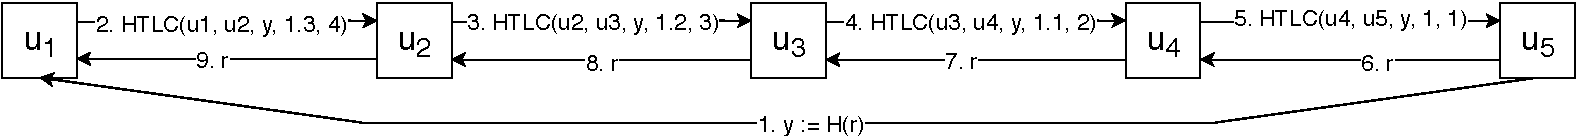
\includegraphics[width=\textwidth]{htlc-figure}
	\caption{An HTLC-based payment in the Lightning Network.}
	\label{fig:htlc}
\end{figure*}

A multi-channel payment leverages a path of channels between a sender and a receiver, who might not share a channel between them.
To initiate a multi-channel payment, the receiver generates a random $r$~and sends its hash $H(r)$~to the sender.
The sender then constructs a path to the receiver and sets up an HTLC with the next node in the path.
The second node sets up an HTLC with the \textit{same} hash value with the third node, and so on.
Finally, the receiver redeems the payment from the last channel by revealing $r$, which allows all involved channels to be updated.

Note that all HTLCs along the path use the same hash value $y=H(r)$ to achieve atomicity.
If the receiver reveals $r$, all channels are updated.
Otherwise, none of them are.

An illustrative example of an HTLC-based payment is depicted in~\cref{fig:htlc}.
Here, the user $u_1$~transfers $1$~coin to $u_5$~using $u_2$, $u_3$~and~$u_4$~as intermediaries.
For that, $u_5$~locally chooses a value $r$~uniformly at random, computes the cryptographic challenge for the HTLC as $y := H(r)$, and sends $y$~to the sender in an \textit{invoice} (step 1).
Then, the payment starts with a commit phase (steps 2-5) where every pair of nodes, starting from the sender, establishes an HTLC using $y$.
After the commit phase is finished, the payment enters the release phase.
Here, the receiver reveals $r$~to $u_4$~to fulfill the contract (step 6), triggering the release phase where every pair of nodes fulfills their contract from the receiver to the sender (steps 6-9).

Intermediaries may charge fees for their forwarding service.
For instance, $u_2$~receives $1.3$~coins but only forwards $1.2$~coins, getting a fee of~$0.1$~coins.
No fees are collected if a payment fails, as all pending balance updates roll back.
In the LN implementations, the fee consists of two parts: a constant \textit{base fee} for each payment and a \textit{fee rate} proportional to the payment value.\footnote{The LN fee structure is different from Bitcoin fees, where the fee is proportional to transaction weight (roughly speaking, size in bytes) but does not account for the transaction value. As of 2019, LN fees are largely non-economical~\cite{Beres2019}.}

The time parameter of the HTLCs along the path decreases to guarantee a safety margin between the timeouts.
For example, the HTLC between $u_1$~and~$u_2$~sets a timeout of four days, whereas the timeout in the HTLC between $u_2$~and~$u_3$~is only three days.
The difference between the timelocks ensures that $u_2$~has enough time to settle the contract with~$u_1$~after receiving $r$~from $u_3$, even if $u_3$~reveals the preimage at the last moment.
We observe an inherent trade-off regarding timeout lengths.
If timeouts are short, a victim of a malicious channel closure may be unable to dispute it if the blockchain is congested at that time.
If timeouts are long, an attacker can route many unsettled payments through a channel and effectively block it until the timelock expires.

Multi-path payments use onion routing to enforce the order of intermediary nodes.
Each intermediary node only knows the immediately previous and next nodes, but not the final sender or receiver and not its position in the path.


\subsubsection*{Channel closure}

A channel is closed when a transaction that spends the output of the funding transaction gets confirmed on-chain.
Channel closure may happen in one of three ways:

\begin{itemize}
	\item Collaborative closure. Alice signals the intent to close the channel, and Bob cooperates in signing the transaction that reflects the latest channel state. Collaborative closure results in one on-chain transaction and imposes no delays. Both parties must be online and cooperating.
	\item Non-cooperative closure without breach. Alice signals the intent to close the channel, but Bob does not respond. In this case, Alice publishes the latest commitment transaction on the blockchain. Bob can redeem his output immediately, but Alice has to wait until a timeout expires. This safety measure allows Bob to broadcast a \textit{justice transaction} if Alice were trying to broadcast an old commitment transaction.
	\item Non-cooperative closure with a breach. Alice broadcasts an old commitment transaction, thus potentially stealing from Bob. If Bob does not react before the timelock on Alice's output expires, Alice can redeem her output, and the channel is closed.\footnote{From the on-chain point of view, a non-disputed non-cooperative close is indistinguishable from a non-cooperative close without a breach. Layer-one does not know whether a commitment transaction is the last one, unless this fact is disputed.} If Bob is online and notices the breach before the timeout, he broadcasts the latest commitment transaction, which allows Bob to spend Alice's output before she can, punishing her for the cheating attempt.
\end{itemize}

This state replacement mechanism makes Lightning superior to earlier payment channel designs.
Lightning channels have an unlimited lifetime (the parties do not have to close the channel if none of them wants to) and support bi-directional payments.
However, the parties must be online to notice potential malicious channel closures and broadcast justice transactions.
LN users may outsource this function to \textit{watchtowers} -- entities that watch the blockchain for malicious channel closures and dispute them on the user's behalf.
Implementing effective, economically incentivized, and privacy-preserving watchtowers in an active area of research~\cite{McCorry2019}.

The LN's revocation technique has proved useful as deterrence against malicious channel closures.
As of July~2019, only $241$~channel closures have been followed by a justice transaction.
This constitutes only $0.7\%$~of channels at that time~\cite{BitMEXLN3}.\footnote{The research is based on the LN's on-chain footprint and may not show the full picture. A non-cooperative closure followed by a justice transaction may also happen without malicious intent, for example, if a channel is incorrectly restored from backup (where Alice's node "forgets" about the latest state and broadcasts an earlier state assuming it is the latest one).}


\subsection{P2P network and path-finding}

Lightning network is \textit{source-routed}.
The sender determines the path to the receiver.
LN nodes gossip about new channels available for routing.
Based on this information, each node maintains a local model of the network graph and uses it to generate routes to the receiver.
The total capacities of public channels are known.
The sender only considers channels with the capacity larger than $x$~for a payment of amount $x$.

However, this is insufficient to prevent routing failures.
The ability of channel parties to send or forward payments is limited by their \textit{local} channel balances.
Consider an example.
After Alice opens a channel with Bob, all funds are initially on her side.
She can send up to the total capacity, but she cannot receive payments.
As the local balances change, the routing capabilities of the channel in both directions also change.

The lack of information about local channel balances makes routing unreliable, especially for larger amounts.
If a payment fails, an error message notifies the sender which channel has failed.
The sender then tries a different route.
The process repeats until the payment succeeds.


\subsection{The future of Lightning}

The future of Lightning depends in part on the planned modifications in the Bitcoin protocol.
Such changes usually take years to implement, test, and roll out.
Let us outline some of the directions for future developments of Lightning.

\paragraph{Schnorr-Taproot}

\textit{Schnorr signatures} is a digital signature algorithm that is considered preferable to ECDSA currently used in Bitcoin\footnote{US patent~\cite{Schnorr1989} covering Schnorr signatures expired in 2008. The patent prevented the implementation of this signature scheme in the original version of Bitcoin.}
In particular, this signature scheme allows for arithmetic on signatures.
In the context of Bitcoin, this makes multi-signatures indistinguishable from signatures with a single signer.
Schnorr signatures are being integrated in Bitcoin as part of a complex \textit{Schnorr-Tapscript-Taproot} update~\cite{Hertig2020}.
In the LN context, Schnorr signatures allow for privacy improvements, making Lightning-related transactions indistinguishable from other transaction types to an external observer.

\paragraph{Eltoo}

\textit{Eltoo}\footnote{Stylized as \textit{eltoo} in the original paper.} is an alternative payment channel proposal proposed in 2018~\cite{Decker2018}.
In Eltoo, intermediary transactions are linked linearly, unlike the LN, where they spend the same funding transaction output.
On channel closure, the final transaction is "re-attached" to the funding transaction's output allowing for more efficient state replacement.

Eltoo requires a new \textit{signature flag} -- \texttt{SIGHASH\_NOINPUT}~\cite{Decker2017}.
A signature flag specifies whether a transaction signature commits to all or only some of the inputs.
Allowing a transaction to \textit{not} commit to any input allows for "re-attaching" it to any compatible output.
If \texttt{SIGHASH\_NOINPUT} is deployed, this replacement mechanism can be used in the LN or a separate payment channel network.


\section{Research directions in payment channel networks}

Multiple research works have shed light on various aspects of payment-channel networks, such as security~\cite{Malavolta2019, Kiayias2019}, liquidity~\cite{Dandekar2011, MorenoSanchez2018, Conoscenti2019}, topology~\cite{Martinazzi2019, Seres2019}, and routing~\cite{Engelmann2017, Prihodko2016, Malavolta2017a, Grunspan2018, Osuntokun2018, Piatkivskyi2018, Roos2018, Sivaraman2018, Bagaria2019, Pickhardt2019, Pickhardt2019a, ZmnSCPxj2019, ZmnSCPxj2019a, ZmnSCPxj2019b}.
Security and privacy are the directions most relevant to our work.

\paragraph{Security}
Payment channel networks operate in a permissionless environment and should be resilient to attacks.
For instance, in the current LN design, no fees are charged if a payment fails, but failed payments consume network resources.
An attacker may leverage this issue to launch a DoS attack.
Various DoS attacks have been described based on route hijacking~\cite{Tochner2019}, depleting channel capacity~\cite{PerezSola2019}, and exceeding the supported number of concurrent in-flight HTLCs~\cite{Mizrahi2020}.

\paragraph{Privacy}
From the privacy point of view, layer-two protocols improve upon layer-one.
L2 protocols do not store transactions in a globally distributed open database available for analysis.
However, multiple weaknesses in LN privacy have been identified.
Payment privacy can be breached due to short routes and strong statistical hints~\cite{Beres2019}.
A potential countermeasure -- adding noise to channel balances -- has been shown ineffective~\cite{Tang2019}.
An attack that allows determining channel balances, similar to our contribution presented in Chapter~\ref{Chapter06LNprobing}, has also been proposed~\cite{HerreraJoancomarti2019}.
A payment channel protocol called Bolt\footnote{Not to be confused with Basics of Lightning Technology (BOLT) -- the Lightning Network specification.} has also been proposed for a privacy-focused cryptocurrency Zcash~\cite{Green2017} and later modified for compatibility with Bitcoin and renamed to zkChannels~\cite{Akinyele2020}.
Lightning network privacy remains an active research area~\cite{Malavolta2017, Kohen2019, Tang2020, Rohrer2020, Kappos2020}.

